% document formatting
\documentclass[10pt]{article}
\usepackage[utf8]{inputenc}
\usepackage[left=1in,right=1in,top=1in,bottom=1in]{geometry}
\usepackage[T1]{fontenc}
\usepackage{xcolor}

% math symbols, etc.
\usepackage{amsmath, amsfonts, amssymb, amsthm}

% lists
\usepackage{enumerate}

% images
\usepackage{graphicx} % for images
\usepackage{tikz}

% code blocks
% \usepackage{minted, listings} 

% verbatim greek
\usepackage{alphabeta}

\graphicspath{{./assets/images/Week 8}}

\title{02-613 Week 8 \\ \large{Algorithms and Advanced Data Structures}}
 
\author{Aidan Jan}

\date{\today}

\begin{document}
\maketitle

\section*{2, 3 - Trees}
A 2, 3-Tree is a search tree where all internal nodes have between 2 and 3 children.  
\begin{itemize}
	\item If there are two children on the node, then the node has \textbf{1 key}, and the left child is smaller than the key, the right child is larger.
	\item If there are three children on the node, then the node has \textbf{2 keys}.  The left child is smaller than both, the middle child is smaller than the second key but larger than the first, and the right child is larger than both.
	\item This tree is always 'balanced'.
\end{itemize}

\begin{center}
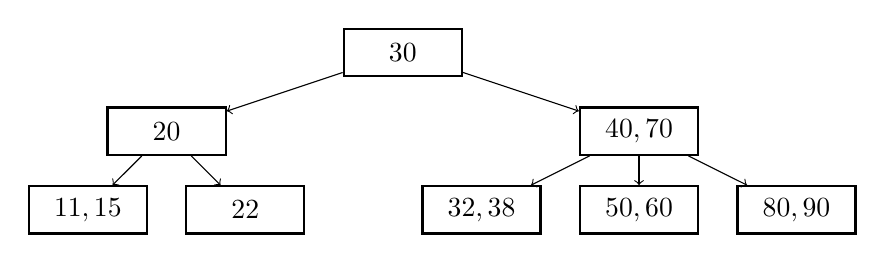
\begin{tikzpicture}
    \node[thick, draw, rectangle, minimum width=1.5cm, minimum height=0.6cm] at (0, 0) (root) {$30$};
    \node[thick, draw, rectangle, minimum width=1.5cm, minimum height=0.6cm] at (-3, -1) (L1N1) {$20$};
    \node[thick, draw, rectangle, minimum width=1.5cm, minimum height=0.6cm] at (3, -1) (L1N2) {$40, 70$};
    \node[thick, draw, rectangle, minimum width=1.5cm, minimum height=0.6cm] at (-4, -2) (L2N1) {$11, 15$};
    %\node[thick, draw, rectangle, minimum width=1.5cm, minimum height=0.6cm] at (-3, -2) (L2N2) {};
    \node[thick, draw, rectangle, minimum width=1.5cm, minimum height=0.6cm] at (-2, -2) (L2N3) {$22$};
    \node[thick, draw, rectangle, minimum width=1.5cm, minimum height=0.6cm] at (1, -2) (L2N4) {$32, 38$};
    \node[thick, draw, rectangle, minimum width=1.5cm, minimum height=0.6cm] at (3, -2) (L2N5) {$50, 60$};
    \node[thick, draw, rectangle, minimum width=1.5cm, minimum height=0.6cm] at (5, -2) (L2N6) {$80, 90$};

    \draw[->] (root) edge (L1N1);
    \draw[->] (root) edge (L1N2);
    \draw[->] (L1N1) edge (L2N1);
    \draw[->] (L1N1) edge (L2N3);
    \draw[->] (L1N2) edge (L2N4);
    \draw[->] (L1N2) edge (L2N5);
    \draw[->] (L1N2) edge (L2N6);
\end{tikzpicture}
\end{center}

\subsubsection*{Insertion}
\begin{itemize}
	\item If we want to insert, we would bubble down from the top to the bottom node, and attempt to add the number as the second key to a node.  
	\item If the chosen node already has two keys, we attempt to push one of the keys to a neighboring node.  The 'pushing to neighbor' operation is called a \textbf{rotation}.
    \item If there are no neighbors to \textbf{overflow} to, then we do a \textbf{split} operation, which a key is pushed up to the parent, and a new node is created.  (We can push up multiple layers!)
    \item If the entire tree is full, then we split the root and add a new node above it, effectively creating a new root.
\end{itemize}
Suppose we wanted to insert $13$.  However, our node is full (and there are neighbors that are not)!  Instead, since we are in a left child, we move the largest value to the root, and push the parent into the right child.
\begin{center}
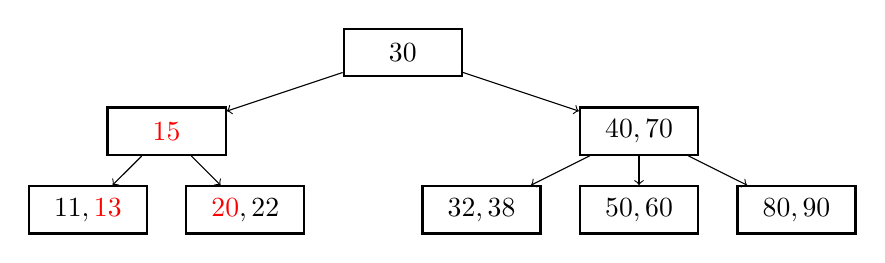
\begin{tikzpicture}
    \node[thick, draw, rectangle, minimum width=1.5cm, minimum height=0.6cm] at (0, 0) (root) {$30$};
    \node[thick, draw, rectangle, minimum width=1.5cm, minimum height=0.6cm] at (-3, -1) (L1N1) {\textcolor{red}{$15$}};
    \node[thick, draw, rectangle, minimum width=1.5cm, minimum height=0.6cm] at (3, -1) (L1N2) {$40, 70$};
    \node[thick, draw, rectangle, minimum width=1.5cm, minimum height=0.6cm] at (-4, -2) (L2N1) {$11, \textcolor{red}{13}$};
    %\node[thick, draw, rectangle, minimum width=1.5cm, minimum height=0.6cm] at (-3, -2) (L2N2) {};
    \node[thick, draw, rectangle, minimum width=1.5cm, minimum height=0.6cm] at (-2, -2) (L2N3) {$\textcolor{red}{20}, 22$};
    \node[thick, draw, rectangle, minimum width=1.5cm, minimum height=0.6cm] at (1, -2) (L2N4) {$32, 38$};
    \node[thick, draw, rectangle, minimum width=1.5cm, minimum height=0.6cm] at (3, -2) (L2N5) {$50, 60$};
    \node[thick, draw, rectangle, minimum width=1.5cm, minimum height=0.6cm] at (5, -2) (L2N6) {$80, 90$};

    \draw[->] (root) edge (L1N1);
    \draw[->] (root) edge (L1N2);
    \draw[->] (L1N1) edge (L2N1);
    \draw[->] (L1N1) edge (L2N3);
    \draw[->] (L1N2) edge (L2N4);
    \draw[->] (L1N2) edge (L2N5);
    \draw[->] (L1N2) edge (L2N6);
\end{tikzpicture}
\end{center}
Suppose we now wanted to add $10$ to the tree.  There is not enough space any of the sister nodes, but there is in the parent.  We therefore need to do a split.
\begin{itemize}
	\item The middle number ($11$) gets pushed up to the parent node, and $10$ and $13$ become their own, separate nodes.
\end{itemize}
\begin{center}
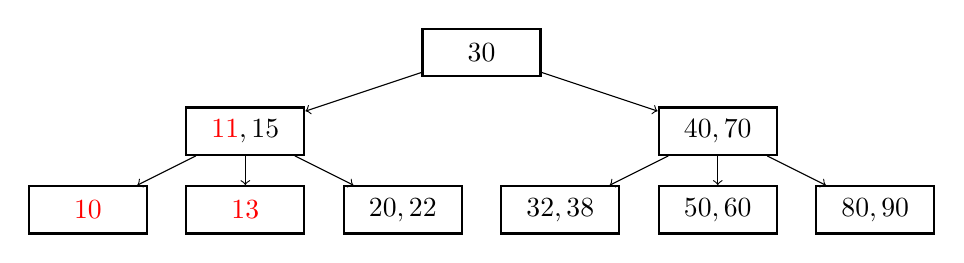
\begin{tikzpicture}
    \node[thick, draw, rectangle, minimum width=1.5cm, minimum height=0.6cm] at (0, 0) (root) {$30$};
    \node[thick, draw, rectangle, minimum width=1.5cm, minimum height=0.6cm] at (-3, -1) (L1N1) {$\textcolor{red}{11}, 15$};
    \node[thick, draw, rectangle, minimum width=1.5cm, minimum height=0.6cm] at (3, -1) (L1N2) {$40, 70$};
    \node[thick, draw, rectangle, minimum width=1.5cm, minimum height=0.6cm] at (-5, -2) (L2N1) {$\textcolor{red}{10}$};
    \node[thick, draw, rectangle, minimum width=1.5cm, minimum height=0.6cm] at (-3, -2) (L2N2) {$\textcolor{red}{13}$};
    \node[thick, draw, rectangle, minimum width=1.5cm, minimum height=0.6cm] at (-1, -2) (L2N3) {$20, 22$};
    \node[thick, draw, rectangle, minimum width=1.5cm, minimum height=0.6cm] at (1, -2) (L2N4) {$32, 38$};
    \node[thick, draw, rectangle, minimum width=1.5cm, minimum height=0.6cm] at (3, -2) (L2N5) {$50, 60$};
    \node[thick, draw, rectangle, minimum width=1.5cm, minimum height=0.6cm] at (5, -2) (L2N6) {$80, 90$};

    \draw[->] (root) edge (L1N1);
    \draw[->] (root) edge (L1N2);
    \draw[->] (L1N1) edge (L2N1);
    \draw[->] (L1N1) edge (L2N2);
    \draw[->] (L1N1) edge (L2N3);
    \draw[->] (L1N2) edge (L2N4);
    \draw[->] (L1N2) edge (L2N5);
    \draw[->] (L1N2) edge (L2N6);
\end{tikzpicture}
\end{center}
Suppose we added a few more numbers so the left subtree of the root is now saturated.
\begin{center}
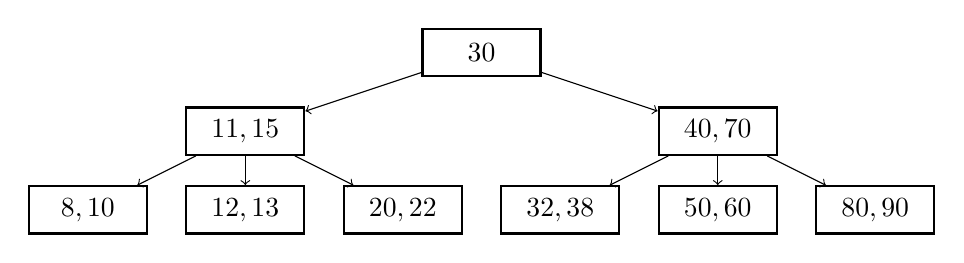
\begin{tikzpicture}
    \node[thick, draw, rectangle, minimum width=1.5cm, minimum height=0.6cm] at (0, 0) (root) {$30$};
    \node[thick, draw, rectangle, minimum width=1.5cm, minimum height=0.6cm] at (-3, -1) (L1N1) {$11, 15$};
    \node[thick, draw, rectangle, minimum width=1.5cm, minimum height=0.6cm] at (3, -1) (L1N2) {$40, 70$};
    \node[thick, draw, rectangle, minimum width=1.5cm, minimum height=0.6cm] at (-5, -2) (L2N1) {$8, 10$};
    \node[thick, draw, rectangle, minimum width=1.5cm, minimum height=0.6cm] at (-3, -2) (L2N2) {$12, 13$};
    \node[thick, draw, rectangle, minimum width=1.5cm, minimum height=0.6cm] at (-1, -2) (L2N3) {$20, 22$};
    \node[thick, draw, rectangle, minimum width=1.5cm, minimum height=0.6cm] at (1, -2) (L2N4) {$32, 38$};
    \node[thick, draw, rectangle, minimum width=1.5cm, minimum height=0.6cm] at (3, -2) (L2N5) {$50, 60$};
    \node[thick, draw, rectangle, minimum width=1.5cm, minimum height=0.6cm] at (5, -2) (L2N6) {$80, 90$};

    \draw[->] (root) edge (L1N1);
    \draw[->] (root) edge (L1N2);
    \draw[->] (L1N1) edge (L2N1);
    \draw[->] (L1N1) edge (L2N2);
    \draw[->] (L1N1) edge (L2N3);
    \draw[->] (L1N2) edge (L2N4);
    \draw[->] (L1N2) edge (L2N5);
    \draw[->] (L1N2) edge (L2N6);
\end{tikzpicture}
\end{center}
Now, what happens if, say, we wanted to add a node with $7$?  None of the leaf nodes or parents have room, so we have to push up to the root.  First, add $7$ to the left most node in the bottom level.  Now we push the middle number up to the parent and split.
\begin{center}
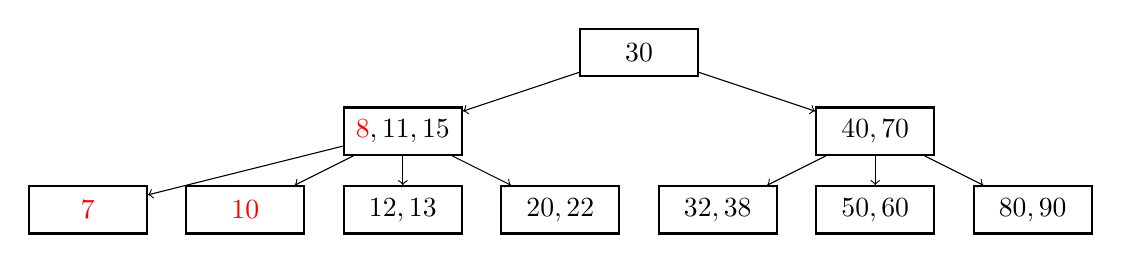
\begin{tikzpicture}
    \node[thick, draw, rectangle, minimum width=1.5cm, minimum height=0.6cm] at (0, 0) (root) {$30$};
    \node[thick, draw, rectangle, minimum width=1.5cm, minimum height=0.6cm] at (-3, -1) (L1N1) {$\textcolor{red}{8}, 11, 15$};
    \node[thick, draw, rectangle, minimum width=1.5cm, minimum height=0.6cm] at (3, -1) (L1N2) {$40, 70$};
    \node[thick, draw, rectangle, minimum width=1.5cm, minimum height=0.6cm] at (-7, -2) (L2N0) {$\textcolor{red}{7}$};
    \node[thick, draw, rectangle, minimum width=1.5cm, minimum height=0.6cm] at (-5, -2) (L2N1) {$\textcolor{red}{10}$};
    \node[thick, draw, rectangle, minimum width=1.5cm, minimum height=0.6cm] at (-3, -2) (L2N2) {$12, 13$};
    \node[thick, draw, rectangle, minimum width=1.5cm, minimum height=0.6cm] at (-1, -2) (L2N3) {$20, 22$};
    \node[thick, draw, rectangle, minimum width=1.5cm, minimum height=0.6cm] at (1, -2) (L2N4) {$32, 38$};
    \node[thick, draw, rectangle, minimum width=1.5cm, minimum height=0.6cm] at (3, -2) (L2N5) {$50, 60$};
    \node[thick, draw, rectangle, minimum width=1.5cm, minimum height=0.6cm] at (5, -2) (L2N6) {$80, 90$};

    \draw[->] (root) edge (L1N1);
    \draw[->] (root) edge (L1N2);
    \draw[->] (L1N1) edge (L2N0);
    \draw[->] (L1N1) edge (L2N1);
    \draw[->] (L1N1) edge (L2N2);
    \draw[->] (L1N1) edge (L2N3);
    \draw[->] (L1N2) edge (L2N4);
    \draw[->] (L1N2) edge (L2N5);
    \draw[->] (L1N2) edge (L2N6);
\end{tikzpicture}
\end{center}
Now the middle number of the parent node is pushed to the root, and we split the tree.
\begin{center}
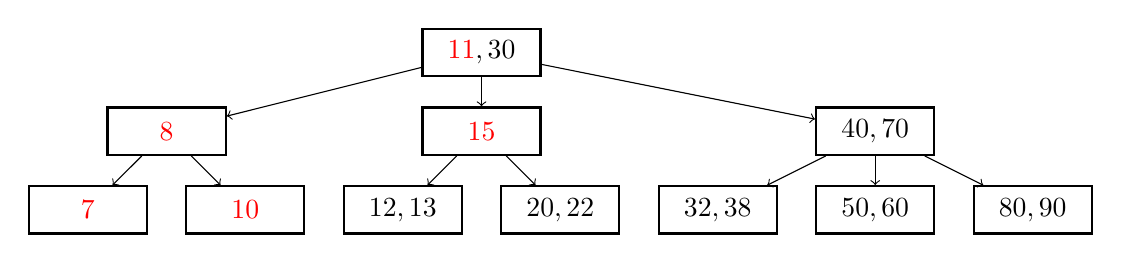
\begin{tikzpicture}
    \node[thick, draw, rectangle, minimum width=1.5cm, minimum height=0.6cm] at (0, 0) (root) {$\textcolor{red}{11}, 30$};
    \node[thick, draw, rectangle, minimum width=1.5cm, minimum height=0.6cm] at (-4, -1) (L1N1) {$\textcolor{red}{8}$};
    \node[thick, draw, rectangle, minimum width=1.5cm, minimum height=0.6cm] at (0, -1) (L1N3) {$\textcolor{red}{15}$};
    \node[thick, draw, rectangle, minimum width=1.5cm, minimum height=0.6cm] at (5, -1) (L1N2) {$40, 70$};
    \node[thick, draw, rectangle, minimum width=1.5cm, minimum height=0.6cm] at (-5, -2) (L2N0) {$\textcolor{red}{7}$};
    \node[thick, draw, rectangle, minimum width=1.5cm, minimum height=0.6cm] at (-3, -2) (L2N1) {$\textcolor{red}{10}$};
    \node[thick, draw, rectangle, minimum width=1.5cm, minimum height=0.6cm] at (-1, -2) (L2N2) {$12, 13$};
    \node[thick, draw, rectangle, minimum width=1.5cm, minimum height=0.6cm] at (1, -2) (L2N3) {$20, 22$};
    \node[thick, draw, rectangle, minimum width=1.5cm, minimum height=0.6cm] at (3, -2) (L2N4) {$32, 38$};
    \node[thick, draw, rectangle, minimum width=1.5cm, minimum height=0.6cm] at (5, -2) (L2N5) {$50, 60$};
    \node[thick, draw, rectangle, minimum width=1.5cm, minimum height=0.6cm] at (7, -2) (L2N6) {$80, 90$};

    \draw[->] (root) edge (L1N1);
    \draw[->] (root) edge (L1N2);
    \draw[->] (root) edge (L1N3);
    \draw[->] (L1N1) edge (L2N0);
    \draw[->] (L1N1) edge (L2N1);
    \draw[->] (L1N3) edge (L2N2);
    \draw[->] (L1N3) edge (L2N3);
    \draw[->] (L1N2) edge (L2N4);
    \draw[->] (L1N2) edge (L2N5);
    \draw[->] (L1N2) edge (L2N6);
\end{tikzpicture}
\end{center}
\begin{itemize}
	\item Alternatively, if the right side of the tree happened to have space, we could do a rotation at the parent level instead of splitting the entire tree at the root.
	\item Also, if the parent is full, we would create a new (empty) node above the parent, and do a split.  This creates a new root with two branches.
\end{itemize}


\section*{a, b - Trees}
The more general case for the $2, 3$-Tree is the $a, b$-Tree
\begin{itemize}
	\item All nodes (except the root and leaves) have between $a-b$ children.
	\item Root has between $2-b$ children.
	\item $a \geq 2$, $b \geq 2a - 1$.
	\begin{itemize}
        \item $a \geq 2$ because otherwise we can't have branches.
	    \item $b \geq 2a - 1$ because otherwise split does not work.
    \end{itemize}
\end{itemize}
Suppose we have a node with $b$ keys and $b + 1$ children, and we need to split.  What do we do?
\begin{itemize}
	\item We would push the middle number up to the parent, and create a new branch on0 the parent.
	\item Now, one node will have $\lceil\frac{b + 1}{2}\rceil$ children, and the other would have $\lfloor \frac{b + 1}{2} \rfloor$ children.
\end{itemize}
In summary:
\begin{center}
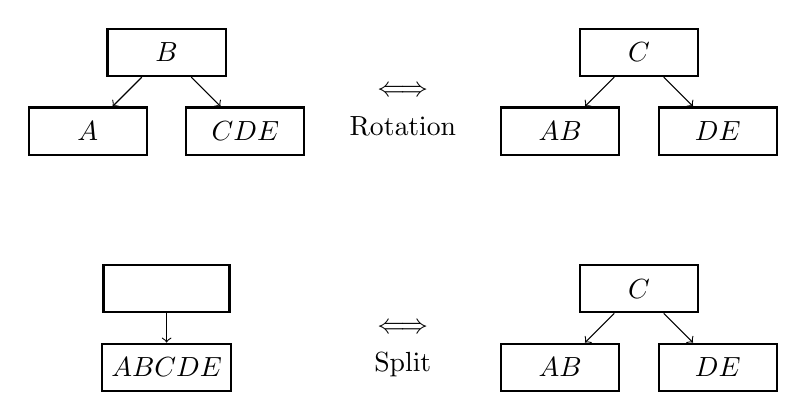
\begin{tikzpicture}
    \node[thick, draw, rectangle, minimum width=1.5cm, minimum height=0.6cm] at (-3, 0) (rootL) {$B$};
    \node[thick, draw, rectangle, minimum width=1.5cm, minimum height=0.6cm] at (-4, -1) (L1N1L) {$A$};
    \node[thick, draw, rectangle, minimum width=1.5cm, minimum height=0.6cm] at (-2, -1) (L1N2L) {$CDE$};
    \node[label=below:{Rotation}] at (0, -0.5) (arrow) {$\Longleftrightarrow$};
    \node[thick, draw, rectangle, minimum width=1.5cm, minimum height=0.6cm] at (3, 0) (rootR) {$C$};
    \node[thick, draw, rectangle, minimum width=1.5cm, minimum height=0.6cm] at (2, -1) (L1N1R) {$AB$};
    \node[thick, draw, rectangle, minimum width=1.5cm, minimum height=0.6cm] at (4, -1) (L1N2R) {$DE$};

    \draw[->] (rootL) edge (L1N1L);
    \draw[->] (rootL) edge (L1N2L);
    \draw[->] (rootR) edge (L1N1R);
    \draw[->] (rootR) edge (L1N2R);

    \node[thick, draw, rectangle, minimum width=1.6cm, minimum height=0.6cm] at (-3, -3) (rootBL) {};
    \node[thick, draw, rectangle, minimum width=1.6cm, minimum height=0.6cm] at (-3, -4) (L1BL) {$ABCDE$};
    \node[label=below:{Split}] at (0, -3.5) (arrow) {$\Longleftrightarrow$};
    \node[thick, draw, rectangle, minimum width=1.5cm, minimum height=0.6cm] at (3, -3) (rootBR) {$C$};
    \node[thick, draw, rectangle, minimum width=1.5cm, minimum height=0.6cm] at (2, -4) (L1N1BR) {$AB$};
    \node[thick, draw, rectangle, minimum width=1.5cm, minimum height=0.6cm] at (4, -4) (L1N2BR) {$DE$};

    \draw[->] (rootBL) edge (L1BL);
    \draw[->] (rootBR) edge (L1N1BR);
    \draw[->] (rootBR) edge (L1N2BR);
\end{tikzpicture}
\end{center}

\end{document}